% Intended LaTeX compiler: pdflatex
\documentclass[10pt,a4paper,UTF8]{article}
\usepackage{zclorg}
\usepackage{tikztheorem}
\author{emacsun}
\date{}
\title{矢量化计算}
\hypersetup{
 pdfauthor={emacsun},
 pdftitle={矢量化计算},
 pdfkeywords={},
 pdfsubject={},
 pdfcreator={Emacs 25.0.50.1 (Org mode 9.1.2)},
 pdflang={English}}
\begin{document}

\maketitle
\tableofcontents
\titlepic{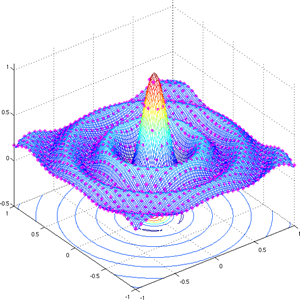
\includegraphics[scale=0.25]{../../img/sinc.PNG}}
\section{简介}
\label{sec:org43fc00d}


吴恩达cosera上机器学习前三次课程作业本身难度不大,很顺利完成,每次作业submit之后都是100points。值得注意的是作业特别强调计算的矢量化。这本身是一件很有意义的事情,因为以 \texttt{for} 或者 \texttt{while} 实现的矢量计算,效率远远不及以矢量本身为操作对象的计算。毕竟 \texttt{for} 或者 \texttt{while} 每次循环执行的是一个矢量元素的计算,而以矢量为操作对象的计算一次就执行了对所有元素的计算。另外,以矢量为操作对象的计算实现起来代码更简短。

这里以第三次作业为例,记录matlab实现矢量化操作的过程。

\section{multi-class classification}
\label{sec:org1a1097b}


由于本文着重强调计算的矢量化,关于什么是 \texttt{multi-class classification} 在这里就不在重述,请参考 \href{week-04-neural-networks.org}{这里} 在作业中我们以5000个手写数字为训练样本,得到一个多类分类器。这5000个样本都是\(20\times 20\)的灰度图像,每一个像素都用一个浮点数表示其灰度。这样一个图像可以用长为400的矢量来表示。在本例中每一个样本是\(X\)的一行。
\lstset{language=matlab,label= ,caption= ,captionpos=b,numbers=none}
\begin{lstlisting}
% Load saved matrices from file
load('ex3data1.mat');
% The matrices X and y will now be in your Octave environment
\end{lstlisting}
通过 \texttt{load} 导入训练样本\(X\)
\begin{equation}
\label{eq:1}
X =
\begin{bmatrix}
- & (x^{(1)})^{T} & - \\
- & (x^{(2)})^{T} & - \\
    &    \vdots     & - \\
- & (x^{(m)})^{T} & -
\end{bmatrix}
\end{equation}
其中\(X\)的每一行都是一个样本,存储着一个数字灰度图像的所有像素构成的矢量,这里每一行都是长为400的矢量。一共\(m\)行,代表着\(m\) 个样本,这里\(m=5000\)。另外导入的数据中还有\(y\),包含了这\(5000\)个样本的正确映射结果。

\subsection{矢量化损失函数}
\label{sec:org6c939db}

logistic回归的损失函数是:
\begin{equation}
\label{eq:2}
J(\theta) = \frac{1}{m} \sum_{i=1}^{m} [ -y^{(i)}\log (h_{\theta}(x^{(i)})) - (1-y^{(i)})\log(1-h_{\theta}(x^{(i)})) ]
\end{equation}

计算损失函数过程中,\(m\)是样本个数,就是说上面的函数把所有的样本都考虑在内了。为了计算求和项的每一个元素,我们需要计算\(h_{\theta}(x^{(i)})\),其中\(h_{\theta}(x^{(i)}) = g(\theta^{T}x^{(i)})\) \(g(z) = \frac{1}{1+e^{-z}}\)。对于\(h_{\theta}(x^{(i)})\)的计算我们可以利用
\begin{equation}
\label{eq:3}
X =
\begin{bmatrix}
- & (x^{(1)})^{T} & - \\
- & (x^{(2)})^{T} & - \\
    &    \vdots     & - \\
- & (x^{(m)})^{T} & -
\end{bmatrix}
\theta =
\begin{bmatrix}
\theta_{0} \\ \theta_{1} \\ \vdots \\ \theta_{n}
\end{bmatrix}
\end{equation}
其中\(X\)的维度是\(5000\times 400\), \(\theta\)的维度是\(400\times 1\),通过计算:
\begin{equation}
\label{eq:5}
X\theta =
\begin{bmatrix}
- & (x^{(1)})^{T}\theta & - \\
- & (x^{(2)})^{T}\theta & - \\
    &    \vdots     & - \\
- & (x^{(m)})^{T}\theta & -
\end{bmatrix}
\end{equation}
\(X\theta\)的维度是\(5000\times 1\),然后根据\textasciitilde{}(\ref{eq:2}) 计算损失函数。

为了防止出现overfitting现象,我们通常需要对损失函数进行正则化:
\begin{equation}
\label{eq:6}
J(\theta) = \frac{1}{m} \sum_{i=1}^{m} [ -y^{(i)}\log (h_{\theta}(x^{(i)})) - (1-y^{(i)})\log(1-h_{\theta}(x^{(i)})) ] + \frac{\alpha}{2m} \sum_{j=1}^{n}\theta_{j}^{2}
\end{equation}
注意这个正则项不包括\(\theta_{0}\),也就是说我们不对偏移项进行正则化。
\subsection{矢量化梯度}
\label{sec:org1678f36}


未正则化的logistic regression的梯度函数是:
\begin{equation}
\label{eq:7}
\frac{\partial J}{\partial \theta_{j}} = \frac{1}{m} \sum_{i=1}^{m}( (h_{\theta}(x^{(i)}) - y^{(i)}) x_{j}^{(i)} )
\end{equation}
我们写出所有\(\frac{\partial J}{\partial \theta_{j}}\):
\begin{equation}
\label{eq:8}
\begin{bmatrix}
\frac{\partial J}{\partial \theta_{0}} \\
\frac{\partial J}{\partial \theta_{1}} \\
\frac{\partial J}{\partial \theta_{2}} \\
\vdots \\
\frac{\partial J}{\partial \theta_{n}}
\end{bmatrix}
=
\frac{1}{m}
\begin{bmatrix}
\sum_{i=1}^{m} (  (h_{\theta}(x^{(i)}) - y^{(i)}) x_{0}^{(i)} )\\
\sum_{i=1}^{m} (  (h_{\theta}(x^{(i)}) - y^{(i)}) x_{1}^{(i)} )\\
\sum_{i=1}^{m} (  (h_{\theta}(x^{(i)}) - y^{(i)}) x_{2}^{(i)} )\\
\vdots \\
\sum_{i=1}^{m} (  (h_{\theta}(x^{(i)}) - y^{(i)}) x_{n}^{(i)} )
\end{bmatrix}

\end{equation}
上式右端可以矢量化为\(\frac{1}{m} \sum_{i=1}^{m}( (h_{\theta}(x^{(i)}) -y^{(i)} )x^{(i})  = \frac{1}{m} X^{T} (h_{\theta}(x) - y)\):

因为这个过程有两个地方体现了矢量化,所以稍微难理解一些。首先从式\textasciitilde{}(\ref{eq:8})到\(\frac{1}{m} \sum_{i=1}^{m}( (h_{\theta}(x^{(i)}) -y^{(i)} )x^{(i)})\) , 我们可以看到\(h_{\theta}(x^{(i)}) - y^{(i)}\)是一个标量 , \(\sum_{i=1}^{m} (  (h_{\theta}(x^{(i)}) - y^{(i)}) x_{0}^{(i)} )\) 实现了 \(m\)个样本与其对应的第\(0\)个feature的点积。依次类推,我们可以得到\(\frac{1}{m} X^{T}(h_{\theta}(x)  -y )\)

对梯度函数的正则化如下:
\begin{eqnarray*}
\frac{\partial J}{\partial \theta_{0}}&=& \frac{1}{m} \sum_{i=1}^{m}( (h_{\theta}(x^{(i)}) -y^{(i)} )x_{0}^{(i)}) \\
\frac{\partial J}{\partial \theta_{j}}&=& \frac{1}{m} \sum_{i=1}^{m}( (h_{\theta}(x^{(i)}) -y^{(i)} )x_{j}^{(i)})  + \frac{\lambda}{m}\theta_{j} \qquad \mathrm{for}\quad j\geq 1\\
\end{eqnarray*}

正则化的矢量化操作比较简单,直接加上\(\frac{\lambda}{m}\theta\),把\(\theta\)的第一项\(\theta_{0}\)赋值为0即可。
\end{document}
